\begin{tcolorbox}[title={Inhalt}]
    \begin{quotation}\noindent
        Im letzten Kapitel wurde bereits ein Einblick in den Aufbau eines neuronalen Netzes gegeben. 
        Dieses Kapitel widmet sich Neuronen, deren Bedeutung in einem Netz und wie diese untereinander verknüpft sind.
        Es wird hier bereits die einfachste Form eines Neuralen Netzwerk vorgestellt.
    \end{quotation}
\begin{itemize} 
    \item Was sind Neuronen
    \item Arten von Neuronen
    \item Funktionsweise
    \item Aktivierungsfunktion
    \item Schichtenmodell
\end{itemize} 
\end{tcolorbox}
\subsection{Was sind Neuronen?}\label{sec:neuronen:was_sind_neuronen}  
Das menschliche Nervensystem besteht aus Neuronen, welche mit Axonen oder Dendriten verknüpft sind. Diese Verbindungen werden auch Synapsen genannt. Die variable Stärke der Synapsen
ermöglichen das Lernen. Dieser biologische Mechanismus wird durch neurale Netze simuliert.\\

\begin{figure}[H]
\begin{subfigure}{0.6\textwidth}
    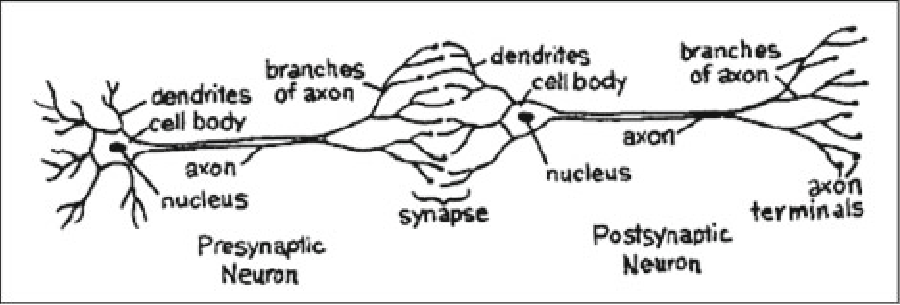
\includegraphics[width=\textwidth]{Sources/01-01_synapse.png}
    \label{Synapse}
    \caption{Synapse}
\end{subfigure}
\begin{subfigure}{0.25\textwidth}
    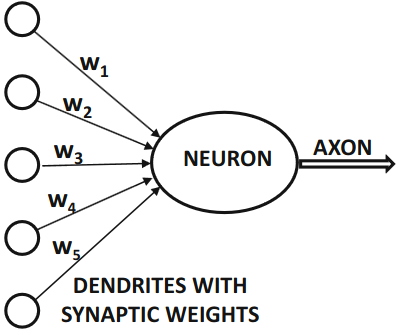
\includegraphics[width=\textwidth]{Sources/01-02_neuron.png}
    \label{Neuron}
    \caption{Neurales Netzwerk}
\end{subfigure}
\caption{Bild aus dem Buch 'Neural Networks and Deep Learning' von Charu C. Aggarwal
}
\end{figure}
\noindent
Ein neuronales Netz besteht aus mindestens einem Neuron. Neuronen sind essentielle Bestandteile von neuralen Netzen. Sie nehmen Eingabedaten entgegen und wandeln diese 
in Ausgabedaten um. Neben den Eingabedaten werden auch Weight-Parameter übergeben, welche die zu berechnenden Werte beeinflussen. Das eigentliche \enquote{Lernen} erfolgt durch diesen 
Einfluss.\cite{CA18}
\subsection{Arten von Neuronen}\label{subsec:neuronen:arten_von_neuronen}
\subsubsection{Input Neuronen}
Input Neuronen erhalten Rohdaten und übergeben diese zusammen mit Weights an die Output Neuronen oder die versteckten Neuronen. Jedes Input Neuron ist mit jedem Neuron aus der nächsten Schicht 
(Hidden oder Output) verknüpft. Eine Aktivierungsfunktions entscheidet, ob das Neuron in der nächsten Schicht aktiviert werden soll. \cite{CA18}
\paragraph{Bias Neuronen}
Das Bias Neuron hat typischerweise den Wert 1. Das Produkt des Bias Neurons und dessen Weight wird auf die Summe der Neuronen aus der Input/Hidden Layer mit auf addiert. Das heißt, dass dieses Neuron
das Ergebnis der Aktivierungsfunktion direkt beinflussen kann. \cite{CA18}
\subsubsection{Versteckte Neuronen}
Versteckte Neuronen befinden sich in den versteckten Schichten zwischen der Eingabe- und der Ausgabeschicht. Diese erhalten Werte von Neuronen aus der vorherigen Schicht und übermitteln diese an die Nächste. \cite{CA18}
\subsubsection{Output Neuronen}
Output Neuronen befinden sich in der letzten Schicht eines neuralen Netzwerks. Auch Output Nodes werden mit Aktivierungsfunktionen aktiviert, wie z.B. der softmax Funktion. \cite{CA18}
